
\chapter{\LaTeX{} Conventions for LBNF/DUNE Documents}
\label{ch:latex-stds}

This chapter provides guidelines on sectioning, inserting figures, tables and references, and formatting numbers and units according to the \LaTeX{} configuration we have set up for LBNF/DUNE documents.

Prepare your section(s) to the level of peer-reviewed publications for an international science journal.
 
Target your introductory section(s) at both scientists from the broad HEP community and at knowledgeable, but not necessarily expert, members of national and international science policy organizations. Recommendation: write the chapter first, then go back and write the introduction to it. It's more likely to be coherent!

Target the body of your section(s) at scientists and engineers from the broader HEP community.


%%%%%%%%%%%%%%%%%%%%%%%%%%%%%%%%%%%%%%%%%%%%%%%%%%%%%%%%%%%%%%%%%%%%
\section{Defined Terms: Macros and the Glossary}
\label{sec:latex-terms}

To enforce consistency among frequently used terms, we have defined \LaTeX{} macros for several names, expressions and parameter values in the file \texttt{common/defs.tex}.  We also use a system called ``DUNE Words'' to enforce consistency of terminology. (Thank you, Brett.)  Terms are defined in the file \texttt{common/glossary.tex}.

%%%%%%%%%%%%%%%%%%%%%%%%%%%%%%%%%%%%
\subsection{The common/defs.tex File}

You may add terms
to this file; this is useful if the name or term is subject
to multiple ``spellings.''  Please add macros carefully, and test them before you commit. 

For example,
\begin{itemize}
\item \anue is written as \verb|\anue|,
\item \dm{21} is written as \verb|\dm{21}|,
\item \sinst{13} is written as \verb|\sinst{13}|,
\item \numutonumu is written as \verb|\numutonumu|,
\item \ptoknubar is written as \verb|\ptoknubar|,
\item the drift velocity parameter value \driftvelocity is written as \verb|\driftvelocity|,
\item \SURF is written as \verb|\SURF|, and
\item \minerva is written as \verb|\minerva|.
\end{itemize}

%%%%%%%%%%%%%%%%%%%%%%%%%%%%%%%%%%%%
\subsection{The common/glossary.tex file}

``If you call it a spade here, call it a spade there.'' We want to enforce consistency in terminology. We do this via a glossary filled with ``DUNE Words.''  This means you should check the \verb|common/glossary.tex| for defined terms and use \verb|\dword{label}| for these terms in your text.

 More information, including variations on \verb|\dword{label}|, is given in Section~\ref{sec:english-terminology}, and the details are explained in Brett's (short) document ``DUNE Words'' at \\
 \url{https://dune.bnl.gov/docs/technical-proposal/dune-words.pdf}.

%%%%%%%%%%%%%%%%%%%%%%%%%%%%%%%%%%%%%%%%%%%%%%%%%%%%%%%%%%%%%%%%%%%%
\section{Numbers and Units}

\textbf{All} numerical quantities expressed as literal number
\textbf{must} have units unless they are inherently unitless.
The international audience demands consistent use of metric units throughout.  Please follow this standard (fully documented at \url{http://mirrors.sorengard.com/ctan/macros/latex/contrib/siunitx/siunitx.pdf}). 

If and only if  a detector component has been purchased or specified using a US/Imperial or another practical non-standard metric unit, then that unit should be listed as well in parentheses that follow (use of the ambiguous but common \si{\kt} is allowed). For example:

``Holes are drilled to a diameter of \SI{0.635}{cm} (\SI{0.25}{in})... The \SI{0.635}{cm} diameter holes are cleaned with...''

In order to enforce consistency the \texttt{siunitx} package is used
and a collection of common units are defined in
\texttt{common/units.tex}.


%%%%%%%%%%%%%%%%%%%%%%%%%%%%%%%%%%%%
\subsection{Bare Numbers}

To enforce consistent writing of numbers please encase them in the
\verb|\num{}| command:

\begin{itemize}
\item ``\num{100}'' is written as \verb|\num{100}|.
\item ``\num{1000}'' is written as \verb|\num{1000}|.
\item ``\num{123.456}'' is written as \verb|\num{123.456}|.
\item ``\num{1+-2i}'' is written as \verb|\num{1+-2i}|.
\item ``\num{3e45}'' is written as \verb|\num{3e45}|.
\item ``\num{.3e45}'' is written as \verb|\num{.3e45}| (keeps the decimal point before the 3).
\item ``\numlist{10;20;30}'' is written as\verb|\numlist{10;20;30}|.
\end{itemize}

%%%%%%%%%%%%%%%%%%%%%%%%%%%%%%%%%%%%
\subsection{Bare Units}

If you need to write a bare unit, one with not associated number, use \verb|\si{}| (lower case ``si''). Some combinations are
defined in the file \texttt{common/defs.tex}.


\begin{itemize}
\item ``\si{\meter}'' is written \verb|\si{\meter}| (The European spelling \verb|\si{\metre}| also works).
\item ``\si{\square\volt\cubic\lumen\per\farad}'' is written \verb|\si{\square\volt\cubic\lumen\per\farad}|.
\item  ``\si{\volt}'' is written \verb|\si{\volt}|.
\item  ``\si{kg.m.s^{-1}}'' is written either as \verb|\si{kg.m.s^{-1}}| or  \verb|\si{\kilogram\meter\per\second}|.
\item  ``\si{kg.m.s^{-1}}'' is written as \verb|\si[per-mode=symbol]{\kilogram\meter\per\second}|. 
\end{itemize}

%%%%%%%%%%%%%%%%%%%%%%%%%%%%%%%%%%%%
\subsection{Numbers with Units}

When a quantity has a unit, write both the numerical part and the unit
using the \verb|\SI{}{}| command like:

\begin{itemize}
\item ``\SI{120}{\GeV}'' is written as \verb|\SI{120}{\GeV}|,
\item ``\SI{4850}{\ft}'' is written as \verb|\SI{4850}{\ft}|,
\end{itemize}

These are defined in the file \texttt{common/units.tex}.

No hyphens shall be used between numbers and units, even if the number-unit is used as an adjective, e.g., ``a 40 kiloton detector.''  (This is a change from past DUNE documents.) 

%%%%%%%%%%%%%%%%%%%%%%%%%%%%%%%%%%%%
\subsection{Common Compound Units}

There are some common units that rather long to type out each time
especially when we require nice formatting. Again, see \texttt{common/units.tex}.

\begin{itemize}
\item ``per \msr'' is written as \verb|per \msr|, and
\item ``exposure in \ktmwyr{}s'' is written as \verb|exposure in \ktmwyr{}s|.
\end{itemize}


%%%%%%%%%%%%%%%%%%%%%%%%%%%%%%%%%%%%%%%%%%%%%%%%%%%%%%%%%%%%%%%%%%%%
\section{Including ``dunefigures''}
\label{sec:latex-figures}

Instead of using the usual \texttt{figure} environment, please use the custom \texttt{dunefigure}
environment in order to provide for a consistent presentation.
The environment is called with one optional and two required
arguments:

\begin{enumerate}
\item An initial, optional short caption to appear in the List Of Figures (LoF), in square brackets. This caption only needs to
identify the figure uniquely, it does not need to describe it fully.
\item A (required) label for referencing. No spaces are allowed in the label. Curly brackets. Start the label with \texttt{fig:} then use the filename of the figure as the rest of the label, (\texttt{image-filename}, below). 
\item The (required) full caption. Curly brackets, again.
\end{enumerate}

Usually the figure contains a graphic via an \texttt{includegraphics} statement.
The filename is assumed relative to a \texttt{graphicspath} as
mentioned in Section~\ref{sec:tech-mainfile} and as such, please (a) put the file in the right place and (b) don't
 specify any directory parts in its name. 
The file's extension may be omitted. Provide an image credit if appropriate. The entry looks like this (make the width/size appropriate for the image):

\begin{verbatim}
    \begin{dunefigure}[optional caption for LoF]{fig:figure-label}
     {required full caption (Credit: xyz)}
    \includegraphics[width=0.8\textwidth]{image-filename}
    \end{dunefigure}
\end{verbatim}

Do not prepend any directory information to the image-filename in the includegraphics line; it will cause an error. The \LaTeX setup that we have already takes care of finding the image. 

Mac users: Please avoid the use of capital letters in graphics filenames; it causes errors that you don't catch when compiling locally on your system. The Mac file systems are not truly case-sensitive, and a mismatch in the capitalization of graphics file names causes problems down the line in the repository.


Remember, ``image-filename'' should match ``figure-label.'' This makes it MUCH easier to find associated references and figures in the \LaTeX{}  source.  Also, we recommend starting the filename with an abbreviated form of the subsystem it relates to, e.g., for the APAs,

\begin{itemize}
\item image filename = apa-frame-and-wires
\item label = fig:apa-frame-and-wires
\item reference = fig:ig:apa-frame-and-wires
\end{itemize}

Example:
\begin{dunefigure}[An aerial photograph of Fermilab]{fig:fermilab-aerial}{An aerial photograph of Fermilab
    showing Wilson Hall and surrounding accelerator rings (Photo: Fermilab
    Visual Media Services).}
  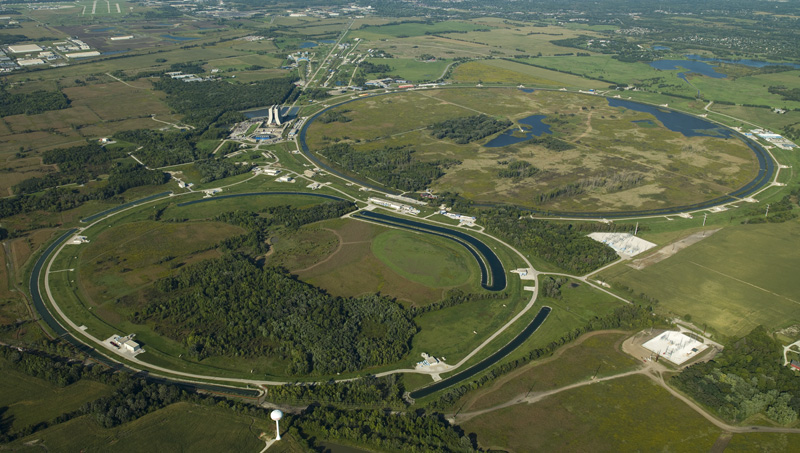
\includegraphics[width=0.8\textwidth]{fermilab-aerial}
\end{dunefigure}


An example can be seen in Figure~\ref{fig:fermilab-aerial}, which is created
with the \LaTeX{} shown in Figure~\ref{fig:aerial-latex}.  Notice that in the reference to the figures, we need to prepend \texttt{fig:} to the label. (See Section~\ref{sec:latex-intra-doc-ref}.)

\begin{dunefigure}[\LaTeX{} source for figure inclusions.]{fig:aerial-latex}{\LaTeX{} source showing how to include Figure~\ref{fig:fermilab-aerial}.}
\begin{verbatim}
    \begin{dunefigure}[An aerial photograph of Fermilab]{fig:fermilab-aerial}
       {An aerial photograph of Fermilab showing Wilson Hall and 
       surrounding accelerator rings (Photo: Fermilab Visual Media Services).}
    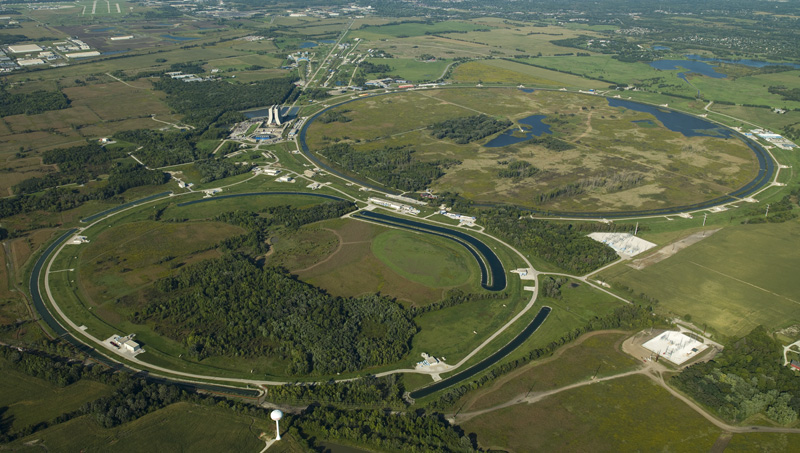
\includegraphics[width=0.8\textwidth]{fermilab-aerial}
    \end{dunefigure}
\end{verbatim}
\end{dunefigure}

See Chapter~\ref{ch:graphics} for guidelines on the graphics files themselves.

\FloatBarrier

%%%%%%%%%%%%%%%%%%%%%%%%%%%%%%%%%%%%%%%%%%%%%%%%%%%%%%%%%%%%%%%%%%%%
\section{Including ``dunetables''}
\label{sec:latex-tables}

Like figures, we use a special environment, \texttt{dunetable} for
tables to achieve a degree of consistency.
This replaces the usual double \texttt{table} + \texttt{tabular} environments.
The \texttt{dunetable} environment takes one optional and three
required arguments:

\begin{enumerate}
\item An initial, optional short caption for the List of Tables (LoT). Square brackets.
\item The tabular column specification. (Curly brackets for the last three items.)
\item A label for referencing. Start the label with \texttt{tab:}. 
\item The full caption.
\end{enumerate}

Inside the actual contents of the table you are required to provide an
initial row containing the headings for the table's rows followed by a
\texttt{toprowrule} macro.
Following every regular row (except the last) you should include a
\texttt{colline} macro.
Both of these take the place of the usual \texttt{hline}.

\begin{dunetable}
[The LoT caption]
{cc}
{tab:example}
{This is a sample table.}
  Rows & Counts \\ \toprowrule
  Row 1 & First \\ \colhline
  Row 2 & Second \\ \colhline
  Row 3 & Third \\ 
\end{dunetable}

\noindent Table~\ref{tab:table-label} is thus made like (arguments can span lines):

\begin{verbatim}
\begin{dunetable}
[The LoT caption]
{cc}
{tab:table-label}
{This is a sample table.}
  Rows & Counts \\ \toprowrule
  Row 1 & First \\ \colhline
  Row 2 & Second \\ \colhline
  Row 3 & Third \\ 
\end{dunetable}

See Table~\ref{tab:table-label}...
\end{verbatim}

The ``cc'' means: ``two columns, both centered.'' You can substitute ``l'' or ``r'' to left- or right-justify a column's contents. Use \verb|p{'width'}| (e.g.,\verb|p{0.2\textwidth}| or \verb|p{5cm}| if you need a column's contents to wrap to multiple lines.

Table~\ref{tab:pdecay} shows a more complex example.
See the source for how it is written.
Note that special column specifications are used.

\begin{dunetable}
[Efficiencies and background rates for nucleon decay modes]
{$L^c^c^c^c}
{tab:pdecay}
{Efficiencies and background rates for nucleon decay channels of interest for a large underground LArTPC, and 
comparison with water Cherenkov detector capabilities}
Decay Mode & \multicolumn{2}{^c}{Water Cherenkov} & \multicolumn{2}{^c}{Liquid Argon TPC} \\
\rowtitlestyle              % ``\rowstyletitle'' is needed here to bold the 2nd row of header text.
& Efficiency & Background & Efficiency & Background \\ \toprowrule
$p \rightarrow K^+ \overline{\nu}$ & 19\% & 4 & 97\% & 1 \\ \colhline
$p \rightarrow K^0 \mu^+$ & 10\% & 8 & 47\% & $<2 $ \\ \colhline
$p \rightarrow K^+ \mu^- \pi^+$ & & & 97\% & 1 \\ \colhline
$n \rightarrow K^+ e^- $ & 10\% & 3 & 96\% & $<2$ \\ \colhline
$n \rightarrow e^+\pi^-$ & 19\% & 2 & 44\% & 0.8 \\
\end{dunetable}

\FloatBarrier



%%%%%%%%%%%%%%%%%%%%%%%%%%%%%%%%%%%%%%%%%%%%%%%%%%%%%%%%%%%%%%%%%%%%
\section{Labels and Intra-document References}
\label{sec:latex-intra-doc-ref}

Assume that any chapter, section or important sub-, subsub- section
or any figure or table environment may need to be referenced
elsewhere in the text. 

Just below a chapter heading and any significant section heading a
label should be added so it can be referenced. Use the defined label in a \verb|\ref{mylabel}| in order to make reference
to the chapter, section, figure, etc.

For example:

\begin{verbatim}
\chapter{A Chapter}
\label{ch:a-chapter}

\section{A Section}
\label{sec:a-section}

\subsection{A Subsection}
\label{sec:a-subsection}

... as described in Chapter~\ref{ch:a-chapter} ... 
or Section~\ref{sec:a-section} ... 
or Section~\ref{sec:a-subsection} ...

\end{verbatim}

When you reference a chapter, section, subsection, figure, table,
etc., capitalize the word ``Chapter'' or whatever it is, e.g., ``as
shown in Section~\ref{sec:tech-mainfile}.''
Use the word ``Section'' even if it's a subsection or subsubsection,
and use the tilde sign to keep the number on the same line as the word
that precedes it.

For figures, the labels and references need to include ``fig:'' before the actual label name, as mentioned in Section~\ref{sec:latex-figures}; for tables, ``tab:'' must be prepended to the label name (see Section~\ref{sec:latex-tables}).


%%%%%%%%%%%%%%%%%%%%%%%%%%%%%%%%%%%%%%%%%%%%%%%%%%%%%%%%%%%%%%%%%%%%
\section{Citations and the Bibliography}
\label{sec:latex-cit}

%%%%%%%%%%%%%%%%%%%%%%%%%%%%%%%%%%%%
\subsection{The Bibliography File Containing the Citations}
\label{sec:latex-bib-file}

For the TDR, we have created the file \texttt{common/tdr-citedb.bib} to contain all the citations. Please read the guidelines at the
beginning of that file. We have left a well-populated \texttt{common/citedb.bib} in the TDR directory in case you want to search for a citation
 that may have appeared in the CDR, or other DUNE/LBNF document.

Note that the bib file is \textbf{not} in \LaTeX{} format and in particular does not
indicate comments via \texttt{\%} characters. (Again, guidelines are in the file itself.)
The
generated bibliography reflects the order in which citations are referenced in the text, not the order of entries in this file.

When adding citations to this file, if possible, copy the BibTeX rendering of the citation from \url{http://inspirehep.net}.

Manual care must be taken to avoid duplication. %\fixme{BV found something; I have to look at it. AH}
Before adding any entry to \texttt{tdr-citedb.bib}, search through it
to ascertain whether the entry you wish to add is already there.

JabRef (\url{http://www.jabref.org/}) is a cross-platform Java GUI that can be used to search bibliographies, possibly investigating duplicities, by working on any loaded .bib file.

%%%%%%%%%%%%%%%%%%%%%%%%%%%%%%%%%%%%
\subsection{Referencing Citations}
\label{sec:latex-ref}

Referencing citations is done like \verb|\cite{strunk}| which gives \cite{strunk}.
To reference multiple citations at the same place, use \verb|\cite{strunk,ref2,ref3}| which gives  [1,2,3].

(Compiling the bibliography entries into the document requires an extra step: run ``bibtex'' on
 guidance.tex, then run pdflatex on it again a couple of times. Otherwise you'll see [?] here 
 and no bibliography entry at the end.) 
The key \texttt{strunk} matches an entry in the \texttt{common/tdr-citedb.bib}
file (as relative to the top-level directory).

%%%%%%%%%%%%%%%%%%%%%%%%%%%%%%%%%%%%%%%%%%%%%%%%%%%%%%%%%%%%%%%%%%%%
\section{Vendors and Trademarks}
\label{sec:trademarks}

Please only reference specific vendors when the particular vendor choice is significant. 
We should use a consistent scheme for these. 
 
Accompany the first mention of a commercial product with a footnote.  This will improve readability by allowing for quick identification of the commercial term in question. 
Do not use the trademark symbol \texttrademark{} or registration mark \textregistered{} in the text, but use it in the footnote where appropriate. Add the footnote only on the first occurrence of the product name in a chapter.
Most commercial product names should be capitalized.
Use a short version of the commercial product name in the text itself.
 
The structure of the footnote should be the following:
Begin with a short descriptive phrase.  Then give the name of the company.  Add \texttrademark{} or  \textregistered{} according to what the company does on their web site. Then provide the company's top-level URL. If an electronic address does not exist, use a physical mailing address. Example:

In your text, write ``The component installation requires one Widgetmaster \\
2000\verb|\footnote{Widgetmastermaker\texttrademark{} Widgetmaster 2000 iron bending machine, | \\
\verb|Widgetmastermaker\texttrademark{} Power Widgets http:widgetmastermaker.com.}| because ...''

%%%%%%%%%%%%%%%%%%%%%%%%%%%%%%%%%%%%%%%%%%%%%%%%%%%%%%%%%%%%%%%%%%%%
\section{Standard \LaTeX{} Sectioning, ``The DUNE Way''!}
\label{sec:latex-sectioning}

Most documents get subdivided into chapters (for larger documents) and/or sections and subsections. Please subdivide according to these standards:

\begin{itemize}
\item A subdivision of a larger portion should have content that relates to some aspect of the larger portion. 
\item  If you create one subdivision, create at least one more. Otherwise, the topic of your one subdivision is (by definition) the same as that of the larger portion.
\item In your \LaTeX{} source, add lines of percent signs (comments) to make it easy to find where sections begin and end, as illustrated in the source for this file. (This really helps the editor!)
\end{itemize}

\begin{verbatim}
%%%%%%%%%%%%%%%%%%%%%%%%%%%%%%%%%%%%%%%%%%%%%%%%%%%%%%%%%%%%%%%%%%%%
\end{verbatim}

Please capitalize all significant words in a heading (this is a change from 
previous DUNE documents).

The following sectioning macros are available, ordered from bigger to smaller:

\begin{verbatim}
\chapter{A Chapter}
\section{A Section}
\subsection{A Subsection}
\subsubsection{A Subsubsection}
\end{verbatim}

We recommend that you stop the subsectioning at this point, but you can go down a couple of levels further.
%Consult with the technical editors if you feel finer grained sectioning is required.
Starting from \verb|\subsection|, this produces the following:

%%%%%%%%%%%%%%%%%%%%%%%%%%%%%%%%%%%%%
\subsection{A Subsection}
\label{sec:latex-sec-sub}

This is a subsection.

%%%%%%%%%%%%%%%%%%%
\subsubsection{A Subsubsection}
\label{sec:latex-sec-subsub}

This is a subsubsection.

%%%%%%%%%%%%%%%%%%%
\subsubsection{A Second Subsubsection}
\label{sec:latex-sec-subsub2}

Remember, if you have one, you need at least one more.

%%%%%%%%%%%%%%%%%%%%%%%%%%%%%%%%%%%%%
\subsection{A Second Subsection}
\label{sec:latex-sub2}

Ditto.
